\documentclass[12pt,a4paper]{report}
\usepackage[latin1]{inputenc}
\usepackage{amsmath}
\usepackage{amsfonts}
\usepackage{amssymb}
\usepackage{makeidx}
\usepackage{graphicx}
\usepackage{lmodern}
\usepackage{kpfonts}
\usepackage[usenames,dvipsnames]{color}
\usepackage[left=2cm,right=2cm,top=2cm,bottom=2cm]{geometry}
\usepackage[dutch]{babel}
\usepackage{listings}
\usepackage{pdfpages}

\begin{document}
\begin{titlepage}

\newcommand{\HRule}{\rule{\linewidth}{0.5mm}} % Defines a new command for the horizontal lines, change thickness here

\center % Center everything on the page
 
%----------------------------------------------------------------------------------------
%	HEADING SECTIONS
%----------------------------------------------------------------------------------------

\textsc{\LARGE Totem Health Patch}\\[1.5cm] % Name of your university/college

%----------------------------------------------------------------------------------------
%	TITLE SECTION
%----------------------------------------------------------------------------------------

\HRule \\[0.4cm]
{ \huge \bfseries Totem Health Patch\\Software Guide}\\[0.4cm] % Title of your document
\HRule \\[1.5cm]

\begin{center}
	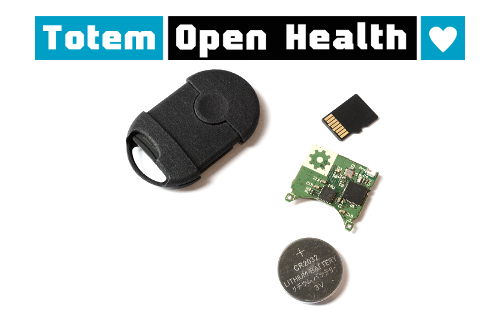
\includegraphics[scale=4.0]{totem}
\end{center} 
%----------------------------------------------------------------------------------------
%	AUTHOR SECTION
%----------------------------------------------------------------------------------------

\begin{minipage}{0.4\textwidth}
\begin{flushleft} \large
\emph{Auteur:}\\
Richard \textsc{den Besten}% Your name
\end{flushleft}
\end{minipage}
~
\begin{minipage}{0.4\textwidth}
\begin{flushright} \large 
\emph{} 
\textsc{} % Supervisor's Name
\end{flushright}
\end{minipage}\\[4cm]

% If you don't want a supervisor, uncomment the two lines below and remove the section above
%\Large \emph{Author:}\\
%John \textsc{Smith}\\[3cm] % Your name

%----------------------------------------------------------------------------------------
%	DATE SECTION
%----------------------------------------------------------------------------------------

{\large \today}\\[3cm] % Date, change the \today to a set date if you want to be precise

%----------------------------------------------------------------------------------------
%	LOGO SECTION
%----------------------------------------------------------------------------------------

%\includegraphics{Logo}\\[1cm] % Include a department/university logo - this will require the graphicx package
 
%----------------------------------------------------------------------------------------

\vfill % Fill the rest of the page with whitespace

\end{titlepage}

\section{Starting Bluetooth Service}
Voor de bluetooth communicatie worden twee bibliotheken gebruikt. De BLEDevice bibliotheek ondersteunt de UARTService die gebruikt wordt als communicatie service. Deze service heeft een Read en Write functie. De UARTService wordt gebruikt om data te ontvangen vanaf een mobiel apparaat. De disconnectionCallback neemt de nodige beslissing om het adverteren te starten wanneer dit kan. Met een verbroken verbinding zal het adverteren weer opnieuw beginnen. TriggerSensorPolling wordt ge"implementeerd om een interrupt uit te voeren. Dit zorgt er voor dat er continu geluisterd kan worden naar de sensoren. De interrupt wordt uitgevoerd wanneer de BLE service iets ontvangt van de master.\\

\begin{lstlisting}
#include "BLEDevice.h"
#include "UARTService.h"

BLEDevice  ble;                                                             

UARTService *uartServicePtr;

static volatile bool  triggerSensorPolling = false;

void disconnectionCallback(Gap::Handle_thandle,Gap::DisconnectionReason_treason)
{
    ble.startAdvertising();
}

\end{lstlisting}
\newpage

\section{Ontvangen data over BLE}
OnDataWritten is de functie die de ontvangen data uit te buffer haalt. Vanaf de master worden er altijd 20 bytes verstuurd. Dit is bepaald om de data gemakkelijk uit elkaar te halen. Elk commando bestaat uit 20 bytes. De const char* incommingdata wordt een 20 bytes lange const char* array met het benodigde commando of data. De   data wordt gecontroleerd met verschillende if statements. Hieronder een lijst met alle commando's waar de software op reageert.\\\\TS--Timestamp-- = 15 bytes voor TS + timestamp\\LDstart = start meting\\ LDstop = stop meting\\ ADaan = acceleratiesensor datalogger aan\\ ADuit = acceleratiesensor datalogger uit\\ GDaan = gyroscoop datalogger aan\\ GDuit = gyroscoop datalogger uit\\ TDaan = temperatuur datalogger aan\\ TDuit = temperatuur datalogger uit\\ HZ--frequentie-- = HZ is commando indicatie met opvolgend de meetfrequentie\\\\Wanneer een commando is gedetecteerd wordt een specifieke FLAG true of false gezet. De firmware weet nu welke commando er uitgevoerd moet worden. Er zijn twee speciale commando's  waar data achter gezet wordt. De timestamp wordt geplaatst achter 'TS'. Dit zijn 13 characters die de timestamp moeten vormen. De timestamp is in milliseconden. Met een for loop maken we een nieuwe char array genaamd timestamp[13]. De meetfrequentie moet op dezelfde manier worden binnengehaald. Deze bevat in totaal 5 characters. De laatste 3 characters vormen de meetfrequentie.

\begin{lstlisting}
void onDataWritten(const GattCharacteristicWriteCBParams *params)                    //UART data ontvangen 
{
    if ((uartServicePtr != NULL) && (params->charHandle == uartServicePtr->getTXCharacteristicHandle())) {
        uint16_t bytesRead = params->len;
        
        const char *incommingData = (char*)params->data;
        
        filter[0] = incommingData[0];
        filter[1] = incommingData[1];
       
        if(std::strcmp(filter, "TS") == 0){
            uint8_t lenght = 2;
            
            for(int i=0; i<=12; i++){
                timestamp[i] = incommingData[lenght];  

                timeparts[i] = incommingData[lenght];

                pc.printf("%d", incommingData[lenght]);
                
                lenght++;
            }
            
            pc.printf("UNIX timestamp in chars: \r\n");
            pc.printf("%s", timestamp);
            
            pc.printf("\r\n");

            pc.printf("UNIX timestamp in integers: \r\n");
            pc.printf("%d", timeparts);

            t.start();
            
        }else if(std::strcmp(incommingData, "LDstart") == 0){
            startFlag = true;
            
        }else if(std::strcmp(incommingData, "LDstop") == 0){
            startFlag = false;
            
        }else if(std::strcmp(incommingData, "ADaan") == 0){
            accFlag = true;
            
        }else if(std::strcmp(incommingData, "ADuit") == 0){
            accFlag = false;
            
        }else if(std::strcmp(incommingData, "GDaan") == 0){
            gyroFlag = true;
            
        }else if(std::strcmp(incommingData, "GDuit") == 0){
            gyroFlag = false;
            
        }else if(std::strcmp(incommingData, "TDaan") == 0){
            tempFlag = true;
            
        }else if(std::strcmp(incommingData, "TDuit") == 0){
            tempFlag = false;
            
        }else if(std::strcmp(incommingData, "HZ") == 0){            
            
        }else if(std::strcmp(incommingData, "") != 0){

        }
        
        ble.updateCharacteristicValue(uartServicePtr->getRXCharacteristicHandle(), params->data, bytesRead);
        triggerSensorPolling = true;
    }
}
\end{lstlisting}
\newpage

\subsection{Timestamp edit}
Om de Unix Timestamp te kunnen gebruiken wordt moet er een fieldconversion plaatsvinden. Zoals hierboven aangegeven wordt alle data ontvangen en geplaatst in een character array. Deze character array moet worden geconverteerd naar een unsigned integer. De Timer die wordt gestart na het ontvangen van de timestamp wordt ontvangen als long integer. De conversie van de Unix Timestamp kan na de conversie opgeteld worden bij de verstreken tijd. De volgende functie maakt van de character array een unsigned integer.\\\\ 

\begin{lstlisting}
unsigned parse_int(const char * p)   //char array converter 
{
    unsigned result = 0;
    unsigned digit;
    while ((digit = *p++ - '0') < 10)
    {
        result = result * 10 + digit;           
    }    
    return result;                   //geef het resultaat terug
}
\end{lstlisting}

Met de volgende code wordt de timestamp vernieuwd. Dit gebeurt altijd vlak voor het schrijven naar de sd-kaart. Op deze manier is de timestamp recent aan de waarden die worden uitgelezen van sensoren. newTimestamp is de unsigned integer die is geconverteerd. De updateTimestamp is de nieuwe tijdwaarde die naar de sd-kaart wordt geschreven.\\\\

\begin{lstlisting}
updateTimestamp = newTimestamp + timer.read_ms();
             
fprintf(fp,"%u", updateTimestamp);
\end{lstlisting}
\newpage

\section{Initialiseren sensoren}
Voordat een meting opgestart kan worden moeten er een aantal configuraties en tests uitgevoerd worden. Wanneer deze tests geslaagd zijn is de firmware klaar voor het adverteren. Dit is het eerste wat de programmatuur uitvoert. Dit is belangrijk omdat er op deze manier gedetecteerd kan worden of er een SD-kaart aanwezig is, er geschreven kan worden naar de SD-kaart, de MPU6050 het juiste device-ID terug geeft en de TMP102 juist geconfigureerd is. De onderstaande functies worden op chronologische volgorde uitgevoerd.\\\\
tempInit();
mpuInit();
sdCardTest();

\begin{lstlisting}
void tempInit(){
    regByte[0] = 0x01;       //configureer register
    regByte[1] = 0x60;       //configureer byte 1
    regByte[2] = 0xA0;       //configureer byte 2
    
    TMP102.write(addr, regByte, 3);    //config-data naar temp sensor
    regByte[0] = 0x00;                 //pointer register 
    TMP102.write(addr, regByte, 1); 
}

void mpuInit(){
    mpu.reset();
    wait(0.2);
    
    mpu.initialize();          //Initialisatie van de MPU6050
    wait(0.2);
    
    bool mpu6050TestResult = mpu.testConnection();
    
    if(!mpu6050TestResult)     //Test resultaat
    {
        while(1){
            debugLed = 1;
            wait(0.2);
            debugLed = 0;
            wait(0.2);
        }
    } else{
    
    }
}

void sdCardTest(){
    CARD_STATUS.mode(PullUp); // Pull up the control line
    wait(0.1); 
    if(CARD_STATUS == CARD_BAY_EMPTY){    
        while(CARD_STATUS == CARD_BAY_EMPTY){
            debugLed = 1;
            wait(0.5);
            debugLed = 0;
            wait(0.5);
        }
        FILE *fp = fopen("/sd/sdtest.csv", "w");
        if (fp != NULL) {
            fprintf(fp, "We're writing to an SD card! SD card can now be used");
            fclose(fp);
        } else {

        } 
    }else{            
        FILE *fp = fopen("/sd/sdtest.csv", "w");
        if (fp != NULL) {
            fprintf(fp, "We're writing to an SD card! SD card can now be used");
            fclose(fp);
        } else {

        }   
    }
    CARD_STATUS.mode(PullDown);
}
\end{lstlisting}
\newpage

\section{Data loggen}
Als de configuratie juist is verlopen en het adverteren is begonnen, kan er verbinding worden gemaakt met het BLE device. De data wordt per sensor gelogd en weggeschreven naar de SD-kaart. Dit gebeurt door middel van de FLAG's die TRUE of FLASE gezet zijn. Wanneer er een FLAG op FALSE staat, wordt er alsnog naar de SD-kaart geschreven. Er zal 'NaN' ingevuld worden op de plek waar heet meting van wordt opgenomen. Voordat de sessie start 'flag' TRUE is gezet, wordt de sessionCounter met 1 opgehoogd. Op deze manier is de character array filenameSessionData bij de start van iedere meting uniek. De filenameSessionData wordt weggeschreven als nieuwe bestandsnaam voor een nieuwe meting. Voor elke meting wordt er een configuratie file aangemaakt. De file verteld welke configuratie er is toegepast bij de desbetreffende meting.\\

\begin{lstlisting}
void sensorRead(){
   if(startFlag == true){
        dataSessionConfig();
        
        char filenameSessionData[23];
        sprintf(filenameSessionData,"/sd/%d-session-data.csv",sessionCounter);
        FILE *fp = fopen(filenameSessionData, "w");

       while(startFlag == true){
            fprintf(fp,(const char *)timestamp);
            pc.printf("%i us\n", t.read_us());
            
            
            if(tempFlag == true){    
                TMP102.read(addr, temp_read, 2);                                    //lees de twee bytes
                temp = 0.0625 * (((temp_read[0] << 8) + temp_read[1]) >> 4);        //convert eer data naar float
                fprintf(fp,";%.2f;", temp);                                         //schrijf float temp naar sd kaart
            }else{
                fprintf(fp,";NaN;");                         
            }
            
            if(accFlag == true){
                mpu.getMotion6(&ax, &ay, &az, &gx, &gy, &gz);                       //haal de data op voor de acc en de gyro
                fprintf(fp,"%d;%d;%d;",ax,ay,az);                 
            }else{
                fprintf(fp,"NaN;NaN;NaN;");
            }
           
            if(gyroFlag == true){               
                fprintf(fp,"%d;%d;%d\n\r",gx,gy,gz);
            }else{
                fprintf(fp,"NaN;NaN;NaN\n\r");                     
            }
        }
        fclose(fp);
        sessionCounter++;
    }
}
\end{lstlisting}

\newpage

\section{Main functie}

De main functie laat een goed overzicht zien van de programmatuur. Na het initialiseren en declareren van globale variabelen en het objecteren van classes en functies wordt de cursor verplaatst naar de main. De main laat duidelijk zien dat de tests en configuratie van de sensoren als eerst wordt uitgevoerd. Vervolgens wordt de BLE communicatie opgezet. BLE wordt ge"initialiseerd en de besproken functie 'onDisconnection' wordt aangeroepen. Na een goede configuratie wordt de set-up voor het adverteren gestart. De advertentie moet een devicename mee geven. In dit geval is het Totem02. Ook de nodige services worden gestart. Waaronder ook de UARTService die gebruikt wordt voor de draadloze communicatie. Na het instellen van een adverteer interval het de BLE advertentie gestart worden. De conditie:
\begin{lstlisting}
triggerSensorPolling && ble.getGapState().connected 
\end{lstlisting} 
is TRUE zolang er niets in de BLE buffer staat. Zo niet, dan wordt door middel van waitForEvent functie geluisterd naar een nieuw inkomend bericht. Deze functie begeeft zich in de bleDevice class.

\begin{lstlisting}
int main(void){
    tempInit();
    mpuInit();
    sdCardTest();
    
    ble.init();
    ble.onDisconnection(disconnectionCallback);                                            // callback funtie voor disconnection
    ble.onDataWritten(onDataWritten);                                                      // callback funtie voor ontvangen bericht

//-------------------------------------------------------------setup adverteren----------------------------------------------------------------------------------
    ble.accumulateAdvertisingPayload(GapAdvertisingData::BREDR_NOT_SUPPORTED| GapAdvertisingData::LE_GENERAL_DISCOVERABLE);             // Indicate that Legacy Bluetooth in not supported
    ble.setAdvertisingType(GapAdvertisingParams::ADV_CONNECTABLE_UNDIRECTED);
    ble.accumulateAdvertisingPayload(GapAdvertisingData::SHORTENED_LOCAL_NAME, (const uint8_t *)"totem02", sizeof("totem02") - 1);
    ble.accumulateAdvertisingPayload(GapAdvertisingData::COMPLETE_LIST_128BIT_SERVICE_IDS, (const uint8_t *)UARTServiceUUID_reversed, sizeof(UARTServiceUUID_reversed));

    ble.setAdvertisingInterval(Gap::MSEC_TO_ADVERTISEMENT_DURATION_UNITS(1000));            //Interval adverteren 1000mS
    ble.startAdvertising();                                                                 //Begin met adverteren

    UARTService uartService(ble);                                                           //Initialiseer pointer naar UART service
                                                                                            //UART service
    uartServicePtr = &uartService;  
         
    while(1){
        if (triggerSensorPolling && ble.getGapState().connected) {
            triggerSensorPolling = true;
            sensorRead();
            
            
            //timer.stop();
            //pc.printf("The time taken was %f seconds\n", timer.read());

        } else {
            ble.waitForEvent();
        }
    }    
}
\end{lstlisting}

\end{document}